\documentclass{article}
\usepackage{graphicx,wrapfig,url,rotating,array}
\usepackage{subcaption}
\textwidth 130mm \textheight 188mm \footskip 8mm
\parindent 0in
%
\title{ESGI132 - Geometric Visualization of a Polygon Area Partitioning}
\author{Todor Balabanov, Stanislav Darachev, Ivan Jordanov,\\
Aleksandar Karakushev, Nikolai Kitanov, Alexander Manov,\\
Georgi Nikolov, Spasimir Nonev, Zdravka Nedyalkova,\\
Emiliyan Rogachev, Natasha Stojkovikj,\\
Petar Tomov, Iliyan Zankinski}
%
\begin{document}
%
\maketitle

\underline{Introduction}
\vspace*{3mm}

In the process of modeling sewerage networks, the main component is the drained area (catchment) from which water is collected to each conduit (pipe). If the area for a single sub-catchment is derived from a mathematical model, we have to create the geometry of that territory, Exactly, in this paper, we want to make geometric visualization for partitioning of a given living area, with respect to the known water debit, relative to each pipe. If each pipe is represent as edges and these edges formed polygon  then our main goal is to make geometric visualization of a polygon area partitioning.
\vspace*{3mm}

\underline{Proposed Solutions}
\vspace*{3mm}

1. Monte Carlo Flooding - With this algorithm the polygon will be divided in irregular shapes. The final result of the algorithm is similar to liquid foolding from different sides.
\begin{figure}[h!]
\centering
\begin{subfigure}{.5\textwidth}
  \centering
  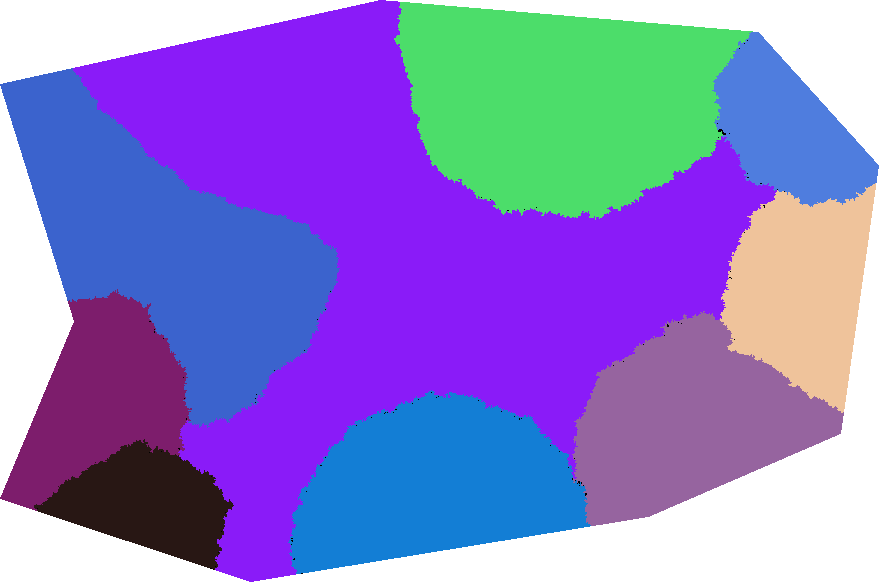
\includegraphics[width=.5\linewidth]{pic08.png}
  \caption{Test case 1.}
  \label{fig:sub7}
\end{subfigure}%
\begin{subfigure}{.5\textwidth}
  \centering
  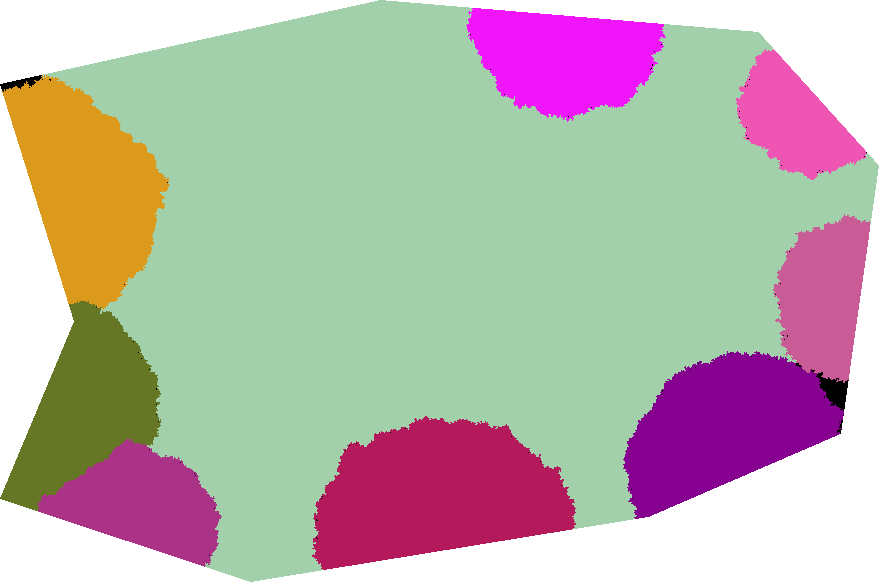
\includegraphics[width=.5\linewidth]{pic09.png}
  \caption{Test case 2.}
  \label{fig:sub8}
\end{subfigure}
\caption{Monte Carlo Flooding algorithm results.}
\label{fig:five}
\end{figure}

2. Percent Distributed Clustering - The given area is divided into a fine grid of pixels. The sides of the polygon are also divided into sixty line segments each. For each pixel of the area the algorithm finds the line segment that gives the lowest value for the distance between the pixel and the line segment multiplied by 100 minus the required percentage of the area: distance * (100 - f(x)). The side that the line segment belongs to is the side that the area taken by the pixel will drain into.
\begin{figure}[h!]
\centering
\begin{subfigure}{.5\textwidth}
  \centering
  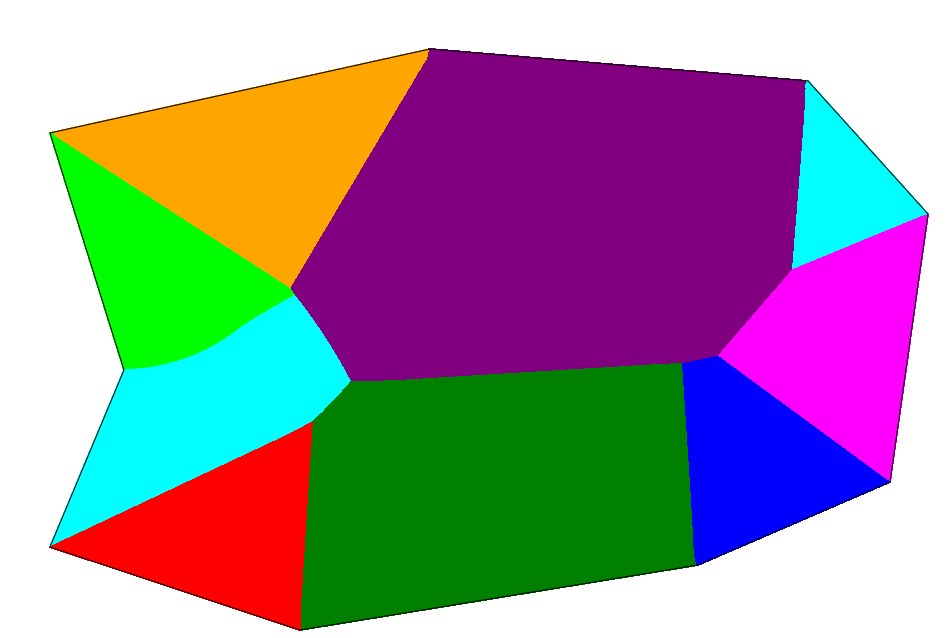
\includegraphics[width=.5\linewidth]{pic10.png}
  \caption{Test case 1.}
  \label{fig:sub9}
\end{subfigure}%
\begin{subfigure}{.5\textwidth}
  \centering
  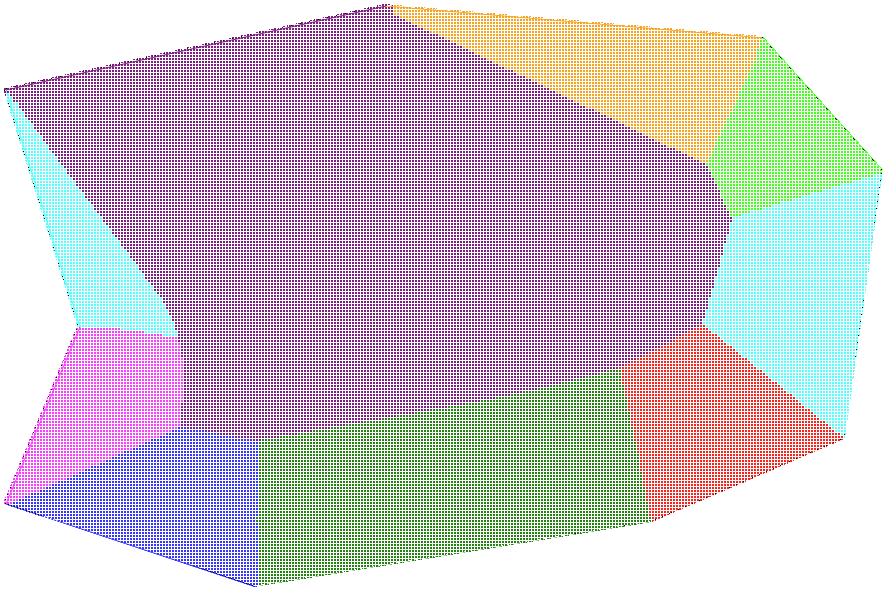
\includegraphics[width=.5\linewidth]{pic11.png}
  \caption{Test case 2.}
  \label{fig:sub10}
\end{subfigure}
\caption{Percent Distributed Clustering algorithm results.}
\label{fig:six}
\end{figure}

3. Offsetting Polygon - The main idea of the offsetting polygon approach is to fill the initial polygon with smaller ones of which each side is parallel to the corresponding one of the initial polygon.
\begin{figure}[h!] 
\centering
\begin{subfigure}{.5\textwidth}
  \centering
  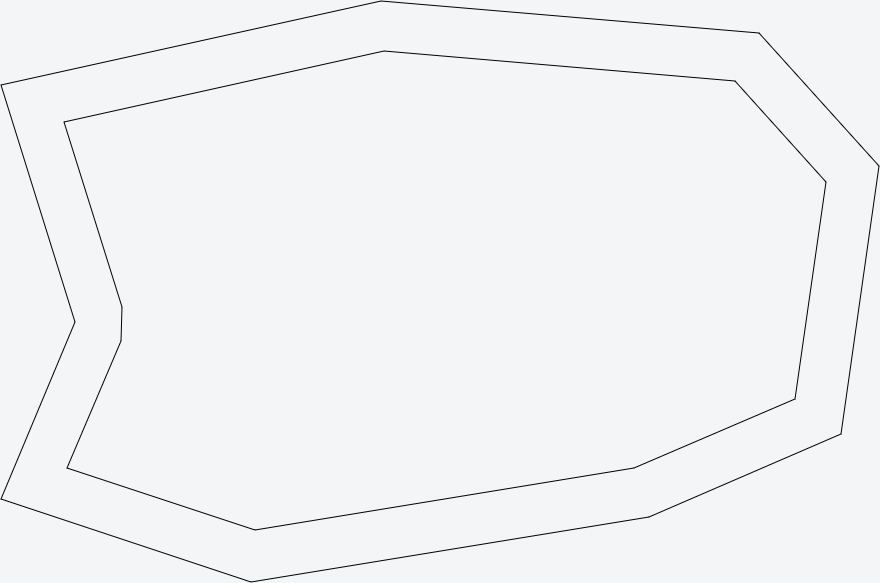
\includegraphics[width=.5\linewidth]{pic12.png}
  \caption{Initial step.}
  \label{fig:sub11}
\end{subfigure}%
\begin{subfigure}{.5\textwidth}
  \centering
  
\includegraphics[width=.5\linewidth]{pic13.png}
  \caption{Final result.}
  \label{fig:sub12}
\end{subfigure}
\caption{Offsetting Polygon algorithm results.}
\label{fig:seven}
\end{figure}
\vspace*{3mm}

\underline{Conclusions}
\vspace*{3mm}

Experimental results show that usage of Percent Distributed Clustering and Offsetting Polygon can produce much better accepted results than Monte Carlo Flooding.
\vspace*{5mm}

\underline{Acknowledgements}
\vspace*{3mm}

Faculty of Mathematics and Informatics, Sofia University St. Kliment Ohridski, Institute of Information and Communication Technologies, Bulgarian Academy of Sciences, Institute of Mathematics and Informatics, Bulgarian Academy of Sciences, European Consortium for Mathematics in Industry, Skyscanner Ltd., Vodostroitelno Predpriatie Ltd., Academy of Music, Dance and Fine Arts - Plovdiv

%
\end{document}
%
% Full addresses of the contact author:
%
% Todor Balabanov
% Institute of Information and Communication Technologies, BAS
% acad. G. Bontchev Str., block 2
% 1113 Sofia, Bulgaria
% todorb@iinf.bas.bg
%